% --------------------------------------------------------------
% This is all preamble stuff that you don't have to worry about.
% Head down to where it says "Start here"
% --------------------------------------------------------------
% Lightly modified from Dana C. Ernst's homework template by Mitchel T. Keller

\documentclass[12pt]{amsart}
 
%\usepackage[margin=1in]{geometry} 
\usepackage{amsmath,amsthm,amssymb}
\usepackage{graphicx}
% If you have issues getting this document to compile BEFORE YOU EDIT
% ANYTHING, then I suggest commenting out the line below, which merely
% changes the document font.
\usepackage{mathptmx}


%% Here are some custom commands relevant to MATH 341
\newcommand{\N}{\mathbb{N}} % \N gets you the "blackboard bold" N
                            % for natural numbers
\newcommand{\Z}{\mathbb{Z}} % \Z gets you the "blackboard bold" Z for
                            % integers 
\newcommand{\R}{\mathbb{R}} % \R gets you the "blackboard bold" R for
% real numbers
\newcommand{\divides}{\mid}

\newenvironment{theorem}[2][Theorem]{\begin{trivlist}
\item[\hskip \labelsep {\bfseries #1}\hskip \labelsep {\bfseries #2.}]}{\end{trivlist}}
\newenvironment{lemma}[2][Lemma]{\begin{trivlist}
\item[\hskip \labelsep {\bfseries #1}\hskip \labelsep {\bfseries #2.}]}{\end{trivlist}}
\newenvironment{exercise}[2][Exercise]{\begin{trivlist}
\item[\hskip \labelsep {\bfseries #1}\hskip \labelsep {\bfseries #2.}]}{\end{trivlist}}
\newenvironment{problem}[2][Problem]{\begin{trivlist}
\item[\hskip \labelsep {\bfseries #1}\hskip \labelsep {\bfseries #2.}]}{\end{trivlist}}
\newenvironment{question}[2][Question]{\begin{trivlist}
\item[\hskip \labelsep {\bfseries #1}\hskip \labelsep {\bfseries #2.}]}{\end{trivlist}}
\newenvironment{corollary}[2][Corollary]{\begin{trivlist}
\item[\hskip \labelsep {\bfseries #1}\hskip \labelsep {\bfseries #2.}]}{\end{trivlist}}

\begin{document}
 
\title{Portfolio\\MATH 467---Introduction to Number Theory}
\author{Your Name Here}
\maketitle

\section{Reflections}

\subsection{Growth as a Mathematician}

% (2 or 3 paragraphs) Describe how you’ve improved as a mathematician
% and student of number theory this semester. Don’t just tell me what you
% learned---focus on one or two important and specific ways that you
% have changed or grown over the course of this semester. Identify at
% least one artifact in your portfolio that illustrates your growth
% area. Explain in the essay how this artifact shows growth in the way
% you’ve described.

Your response here.

\subsection{Definitions}

% (2 or 3 paragraphs) Give a clear, thorough, and general explanation
% of the role of definitions in mathematics. Include: What are
% definitions? Why are they necessary? Where do they come from? Are
% definitions ``true''? Identify an artifact that illustrates the
% importance and use of definition(s), and explain how they are used in
% it. Be specific.

Your response here.

\subsection{Building Connections}

% (2 or 3 paragraphs) Definitions are a central part of mathematics, as
% you have expressed above. However, one of the things we have worked on
% this semester is building skills to see how to leverage both
% definitions and theorems we have already proved when we are attempting
% to prove another theorem. Discuss your journey through connecting
% ideas in this course. Identify one or more artifacts that illustrates
% your growth in this regard. This could include two proofs of the same
% theorem or two different theorems where the proofs you include show
% growth and development in your proof-writing.

Your response here.

\subsection{Speed Round}
  % Turn each of the questions below into a one-sentence statement
  % that includes a brief explanation. Delete the question and replace
  % it with your response, but phrase so I can tell what the question
  % is. For example, "The most difficult part of the class for me was
  % ___ because ___."
  \begin{enumerate}
  \item What was the most difficult part of the class for you?
    You can list a general topic, a specific proof, a type of work we
    did, etc. Tell me why! 
  \item What was the easiest part of the class for
    you? Tell me why! 
  \item What part of class surprised or interested you the
    most? Why? One sentence!
  \end{enumerate}

\section{Artifacts with Commentary}

% Include at least eight artifacts from your work this semester. Some of
% these artifacts will be included in support of your reflections in the
% first section of your portfolio. The others will be artifacts that you
% choose to demonstrate your growth throughout the course of the
% semester. For each artifact that you include, write a couple of
% sentences explaining what that artifact demonstrates about your
% development as a mathematician in this course. (If you include an
% artifact to support a response in the Reflections section, you may
% just write a sentence here stating which response the artifact relates
% to.)

% What is an artifact? For this portfolio, an artifact is a single
% theorem as well as your proof of it (or possibly multiple proofs of a
% single theorem, but a theorem with two proofs is a single
% artifact). You may choose to include photographs/scans of handwritten
% work from a class prep, Test I, or Test II for at most two of your
% eight artifacts. If you do this, then you are also expected to type an
% improved version of the proof for that artifact. This could be based
% on a class presentation or conversations with me or classmates. If you
% include work from a test, the improved version CANNOT be just typing
% up the proof in my solutions. My suggestion is that if you pick a
% problem from a test, then you should wait at least 48 hours between
% looking at my solutions and writing up the improved version of a proof
% for your portfolio. At least six of your artifacts will be theorems
% and proofs from weekly homework. Don't just choose the ones you got
% great grades on! This portfolio is about making an honest reflection
% on your growth and development as a mathematician in this course. Part
% of such a reflection is being willing to show work from early in the
% semester that you look at in December and think ``Wow, I was such a
% beginner when I wrote that!'' Pair that sort of proof with something
% from later in the course that you believe shows your growth and
% development as a mathematician and tell me your personal story from
% this course. (You might also revise a proof that wasn't so great to
% show your progress and explain what experiences helped you improve
% so that you could write that revised version.)

% The command below shows how to include handwritten work, which I
% have chosen to center with the center environment. PDF and
% JPEG should both include well, but other formats probably won't
% work. Notice that I don't need to put the file extension on (but you
% can if you run into issues). You can adjust the 0.5 to make things
% larger or smaller (or just use width=\linewidth to make the image
% included be the width of the line.
\begin{center}
  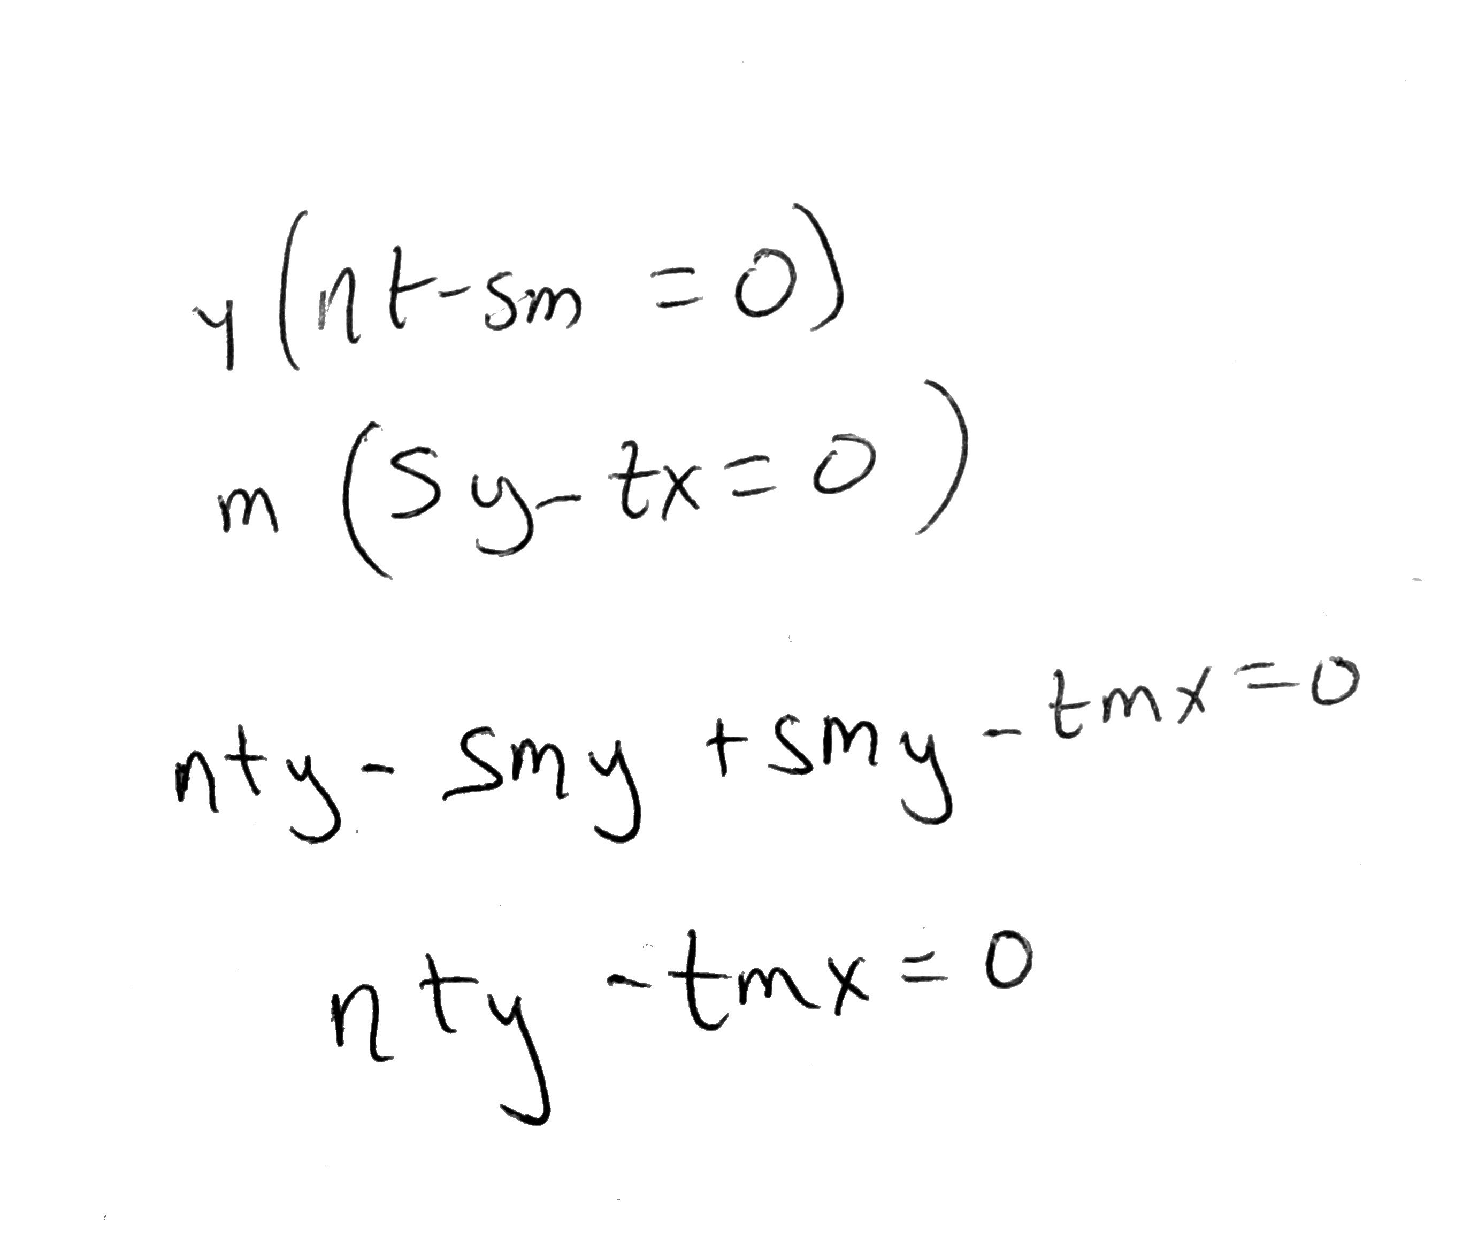
\includegraphics[width=0.5\linewidth]{scratch}
\end{center}
\end{document}
